\chapter{Schematy płytek drukowanych}
\label{boards}

\section{Urządzenie deaktywujące}

Urządzenie deaktywujące powinno zawsze towarzyszyć osobie upoważnionej do uruchomienia pojazdu. Biorąc pod uwagę przykład zastosowania urządzenia we flotach pojazdów, można zauważyć, że zazwyczaj do pojazdu nie jest przypisana jedna osoba, lecz może być on używany przez wielu kierowców. Stąd też logicznym staje się wniosek, że urządzenie nie może być przyporządkowane do kierowcy, lecz do pojazdu. Idealnym rozwiązaniem wydaje się umieszczenie go przy kluczykach lub karcie umożliwiającej uruchomienie pojazdu. Z tego powodu ważne stają się wymiary samego urządzenia. Nie powinno być ono zbyt grube, aby nie przeszkadzało w kieszeni, ani zbyt duże, aby nie obijało się o nogi, a tym samym nie rozpraszało kierującego w trakcie jazdy.
Wymiary płytki urządzenia deaktywującego wynoszą 32 mm x 43 mm.

Ze względu na prostotę konstrukcji, składa się ona z niewielu modułów. Na górnej warstwie płytki (stronie elementów) znajduje się mikrokontroler nRF52832 wraz z anteną 2,4 GHz ISM do komunikacji poprzez Bluetooth Low Energy. Dodatkowo, znajdują się tam: złącze do programowania, złącze debugowe oraz antena NFC, zwizualizowana jako koło koloru niebieskiego. Górną warstwę płytki przedstawiono na rysunku \ref{fig:image_key_tag_top_board}.

Centralne miejsce na dolnej warstwie płytki (stronie lutowania) zajmuje bateria litowa CR2032, która zapewnia kilkuletnią pracę dezaktywatora. Posiada ona średnicę 20 mm oraz grubość 3,2 mm. Mniejsze baterie oferują mniejszą pojemność, a także większy opór wewnętrzny co zwiększa straty energetyczne. Wygląd oraz wizualizację dolnej warstwy płytki przedstawiono na rysunku \ref{fig:image_key_tag_bottom_board}.

\begin{figure}[H]
\centering
	\subfloat[Wygląd górnej warstwy płytki]{
		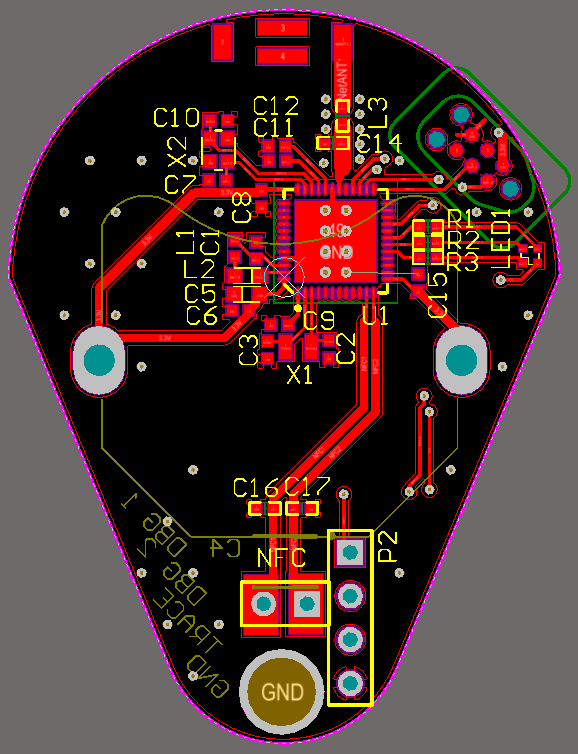
\includegraphics[width=6cm]{img/board_layouts/key_tag_top.png}
	}
	\qquad
	\subfloat[Wizualizacja górnej warstwy płytki]{
		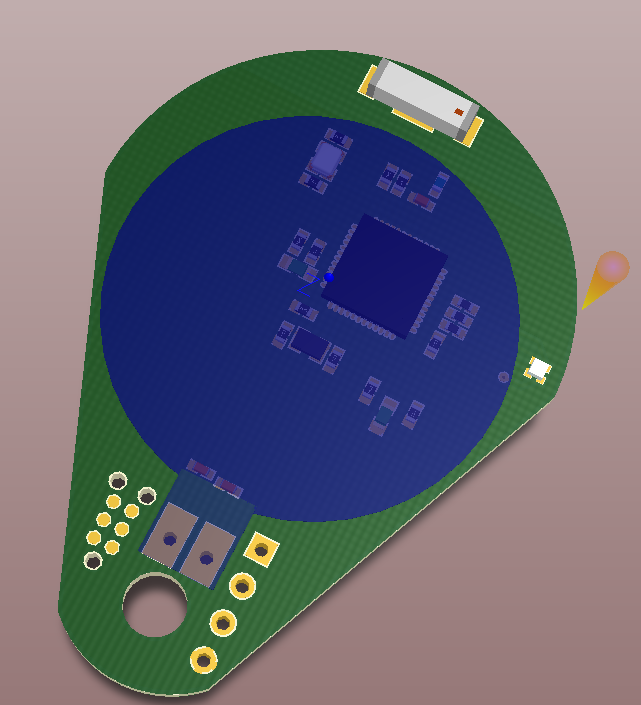
\includegraphics[width=7.1cm]{img/board_layouts/key_tag_visualization_top.png}
	}
	
	\caption{Wygląd górnej warstwy płytki urządzenia deaktywującego oraz jej wizualizacja. \\ Źródło: Opracowanie własne.}
	\label{fig:image_key_tag_top_board}
\end{figure}

\begin{figure}[H]
\centering
	\subfloat[Wygląd dolnej warstwy płytki]
	{
		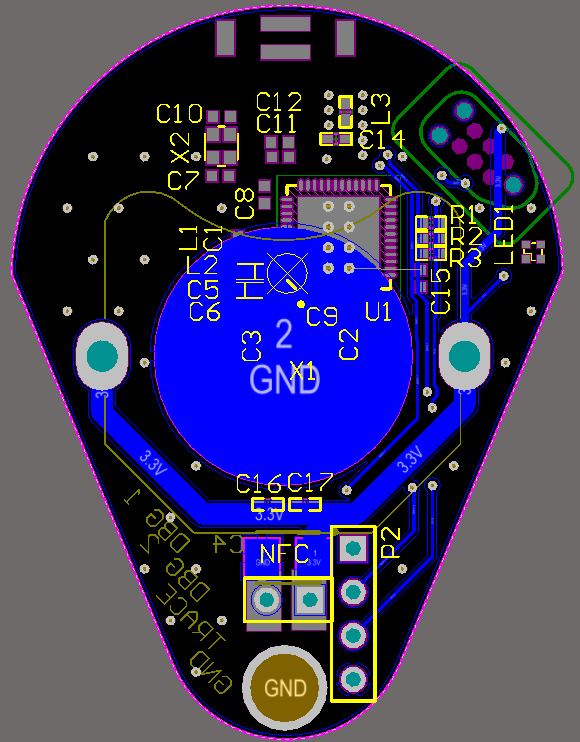
\includegraphics[width=6cm]{img/board_layouts/key_tag_bottom.png}
	}
	\qquad
	\subfloat[Wizualizacja dolnej warstwy płytki]
	{
		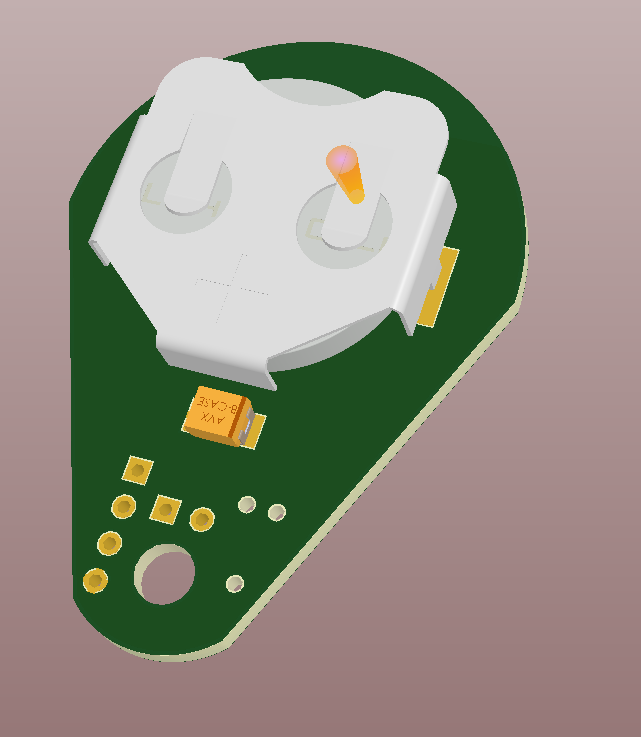
\includegraphics[width=7.1cm]{img/board_layouts/key_tag_visualization_bottom.png}
	}
	
	\caption{Wygląd dolnej warstwy płytki urządzenia deaktywującego oraz jej wizualizacja. \\ Źródło: Opracowanie własne.}
	\label{fig:image_key_tag_bottom_board}
\end{figure}

\section{Urządzenie lokalizujące}

Płytka urządzenia lokalizującego jest znacznie bardziej skomplikowana. \linebreak Ma wymiary 50 mm x 50 mm, co powinno umożliwić jej łatwe ukrycie (na przykład pod kokpitem). Wygląd i wizualizację urządzenia przedstawiono na rysunkach \ref{fig:image_mainboard_top_board} oraz \ref{fig:image_mainboard_bottom_board}.

Ze względu na użycie kilku układów radiowych, wykorzystujących częstotliwości od \linebreak 13,56 MHz (NFC), poprzez 900 MHz/ 1800 MHz (GSM) i 1575,42 MHz (GPS)\linebreak aż po 2,4 GHz (Bluetooth), a także przetwornicy impulsowej o znacznym szczytowym natężeniu prądu (aż do 1,5 A), niezbędne jest odpowiednie rozłożenie elmentów na płytce, które zminimalizowałoby ich wzajemny wpływ. W związku z tym, postanowiono umieścić kluczowe elementy zasilające oraz radiowe w rogach płytki, co maksymalizuje wzajemne odległości. W ten sposób, w lewym górnym rogu płytki umieszczono złącza zasilania, w prawym górnym - cewkę indukcyjną, stanowiącą główny element impulsowej stabilizacji napięcia. Cewka ta stanowi główne źródło zakłóceń sygnałów. W lewym dolnym rogu znajduje się antena Bluetooth Low Energy, natomiast w prawym dolnym rogu - złącze anteny GPS. 

Przewody anten GPS oraz GSM są dodatkowo ekranowane, dzięki czemu znacznie zmniejszona jest podatność tych sygnałów na zakłócenia w trakcie przepływu od anteny do płytki. Jednakże na samej płytce sygnały te nie posiadają ekranu elektromagnetycznego, przez co są podatne na szumy. Z tego względu niezbędna jest minimalizacja długości ścieżek między złączem anteny oraz wejściami układów. W dodatku, sygnał GPS stanowi najsłabszy ze wszystkich sygnałów radiowych, wykorzystywanych w urządzeniu, przez co niezbędne staje się  jak największe oddalenie toru GPS od pozostałych układów. Ze względu na fakt, iż sygnał GSM ma znacznie większą moc, przez co jest mniej podatny na zakłócenia, jego tor radiowy znajduje się na środku prawego boku płytki, bliżej cewki indukcyjnej przetwornicy impulsowej. 

Wszystkie sygnały radiowe są sygnałami analogowymi. Są one podatne na zjawisko odbicia fali elektromagnetycznej, które polega na odbiciu sygnału na końcu przewodu, bądź ścieżki elektrycznej i nałożeniu się na sygnał pierwotny. Wprowadza to dodatkowe zakłócenia w transmisji sygnału, a spowodowane jest niedopasowaniem impedancji toru transmisyjnego. Aby zminimalizować ten efekt, należy zaprojektować ścieżki po których przesyłany jest sygnał wysokiej częstotliwości tak, aby miały odpowiednią impedancję, zgodną z impedancją anteny. Dokonuje się to poprzez dobór grubości (wynika ona z grubości warsty miedzi, zazwyczaj 35 $\mu m$) oraz szerokości (wybór pod kątem optymalnego zużycia miejsca na PCB) ścieżek radiowych. Na podstawie tak wyznaczonych parametrów wylicza się ich niezbędną długość ścieżki, aby osiągnąć założoną impedancję. W przypadku sygnałów GPS, GSM oraz Bluetooth wynosi ona 50 $\Omega$. Ostateczną impedancję, uwzględniającą pojemności i indukcyjności pasożytnicze między ścieżkami, zmierzoną po złożeniu płytki można jeszcze skorygować poprzez dobór elementów w filtrach przyantenowych (filtry: C45, R21, C47 oraz C44, R22, C46). Dodatkowo, ścieżki wysokiej częstotliwości prowadzi się łagodnymi łukami, bez ostrych załamań, które mogłyby zwiększających pojemność, a tym samym mogących zmienić impedancję. 

W dodatku, w trakcie projektowania urządzenia należy pamiętać o wysokim chwilowym poborze prądu. Z tego względu, trzeba zaprojektować odpowiednio grube ścieżki zasilające. Jest to istotne z dwóch powodów. Pierwszym z nich jest rezystancja ścieżki.

\begin{equation}
 R = \rho \cdot l / S 
 \label{eq_pcb_wire_resistance}
\end{equation}

gdzie:

R - oporność ścieżki,

$\rho$ - oporność właściwa materiału, z którego wykonano ścieżkę,

l - długość ścieżki,

S - powierzchnia (liczona jest jako iloczyn grubości i szerokości) ścieżki,

Jak widać, im większa szerokość ścieżki, tym większa jej powierzchnia, a więc mniejsza rezystancja. Im mniejsza rezystancja, tym straty napięcia na samej ścieżce będą mniejsze.

\begin{equation}
 U = R \cdot I
 \label{eq_voltage_drop_on_pcb_wire} 
\end{equation}

 gdzie:
 
 U - strata napięcie na ścieżce,
 
 R - opór ścieżki,
 
 I - prąd płynący przez ścieżkę
 
\clearpage
Drugi przypadek wynika niejako z pierwszego. Gdy opór ścieżki jest zbyt duży, w momencie zwiększonego poboru prądu, energia tracona w ścieżce może być tak duża, że ulega ona zniszczeniu. Aby się przed tym ustrzec, ścieżki zasilające mają grubość 2 mm, co pozwala na przepływ prądu o wartości około 3,5 A w temperaturze otoczenia 20$\deg$C. Ze względu jednak na fakt, iż główne obciążenie urządzenia stanowi prąd chwilowy, trwający bardzo krótko, średnie natężenie prądu będzie dużo niższe od tej wartości. Szerokość ścieżek została dobrana z zapasem tak, aby nie uległy one przepaleniu przed zadziałaniem bezpiecznika zwłocznego. Tabela zestawiająca zależność między grubością ścieżek na płytce PCB od wartości maksymalnego dopuszczalnego prądu ciągłego, przepływającego przez nią, przedstawiono na rysunku \ref{fig:image_pcb_wire_thickness}.

\begin{figure}[H]
	\centering
	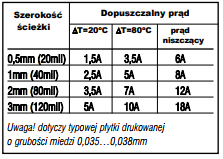
\includegraphics[width=8cm]{img/board_layouts/pcb_wire_thickness.png}
	\caption{Tabela opisująca zależność pomiędzy grubością ścieżek, a maksymalnym dopuszczalnym natężęniem prądu. Źródło: \cite{pcb_wire_thickness}.}
	\label{fig:image_pcb_wire_thickness}
\end{figure}
 

\begin{figure}[H]
\centering
	\subfloat[Wygląd górnej warstwy płytki]{
		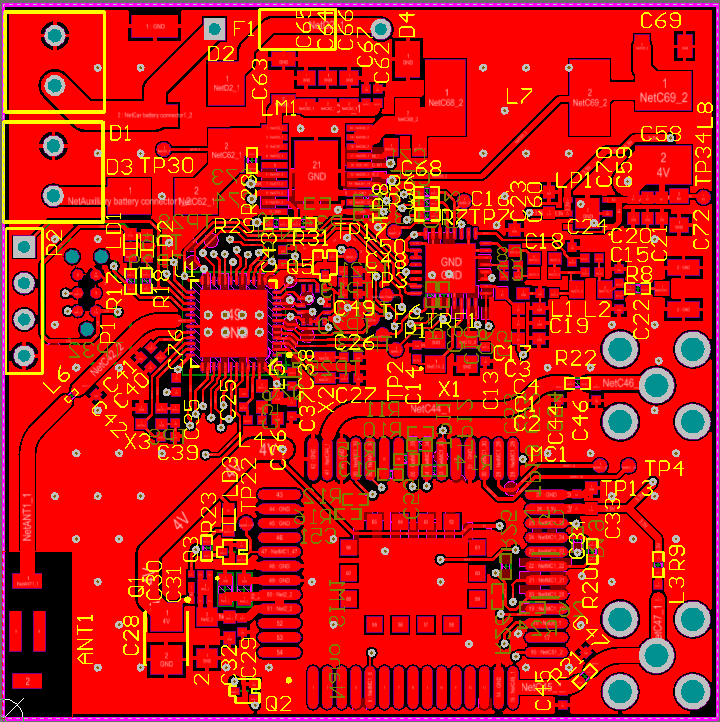
\includegraphics[width=11cm]{img/board_layouts/mainboard_top.png}
	}
	\qquad
	\subfloat[Wizualizacja górnej warstwy płytki]{
		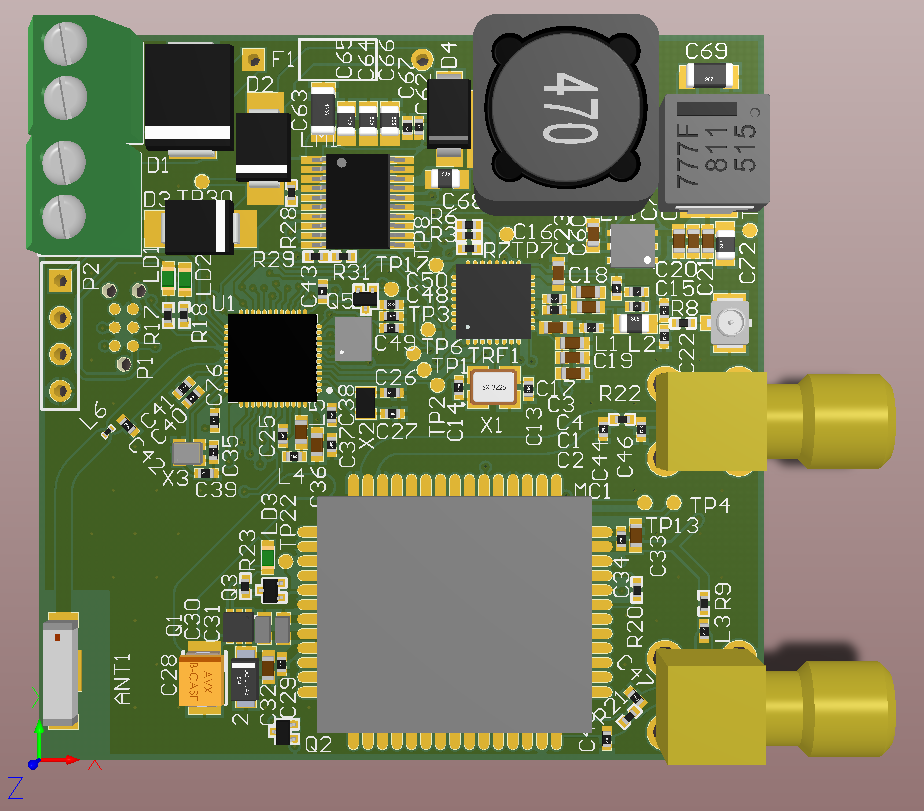
\includegraphics[width=11cm]{img/board_layouts/mainboard_visualization_top.png}
	}
	
	\caption{Wygląd górnej warstwy płytki urządzenia lokalizującego oraz jej wizualizacja. \\ Źródło: Opracowanie własne.}
	\label{fig:image_mainboard_top_board}
\end{figure}

\begin{figure}[H]
\centering
	\subfloat[Wygląd dolnej warstwy płytki]
	{
		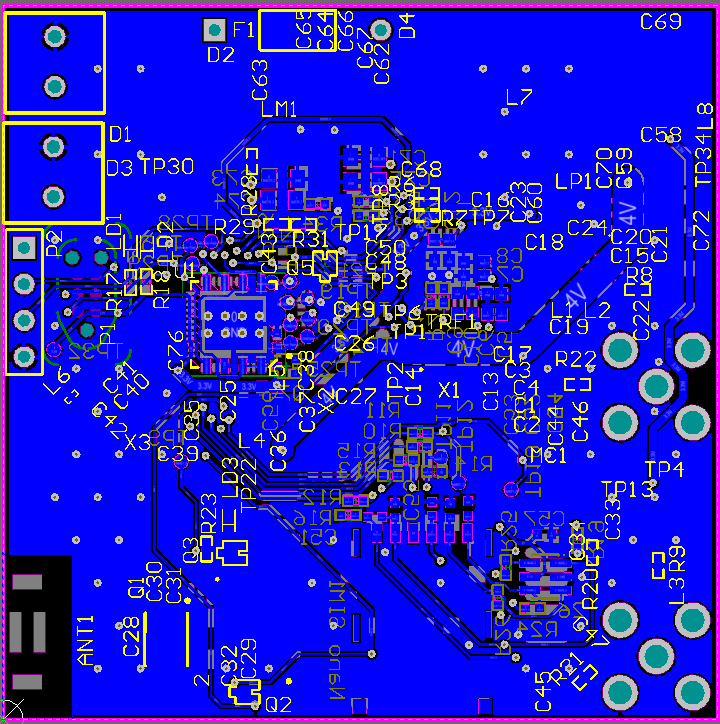
\includegraphics[width=11cm]{img/board_layouts/mainboard_bottom.png}
	}
	\qquad
	\subfloat[Wizualizacja dolnej warstwy płytki]
	{
		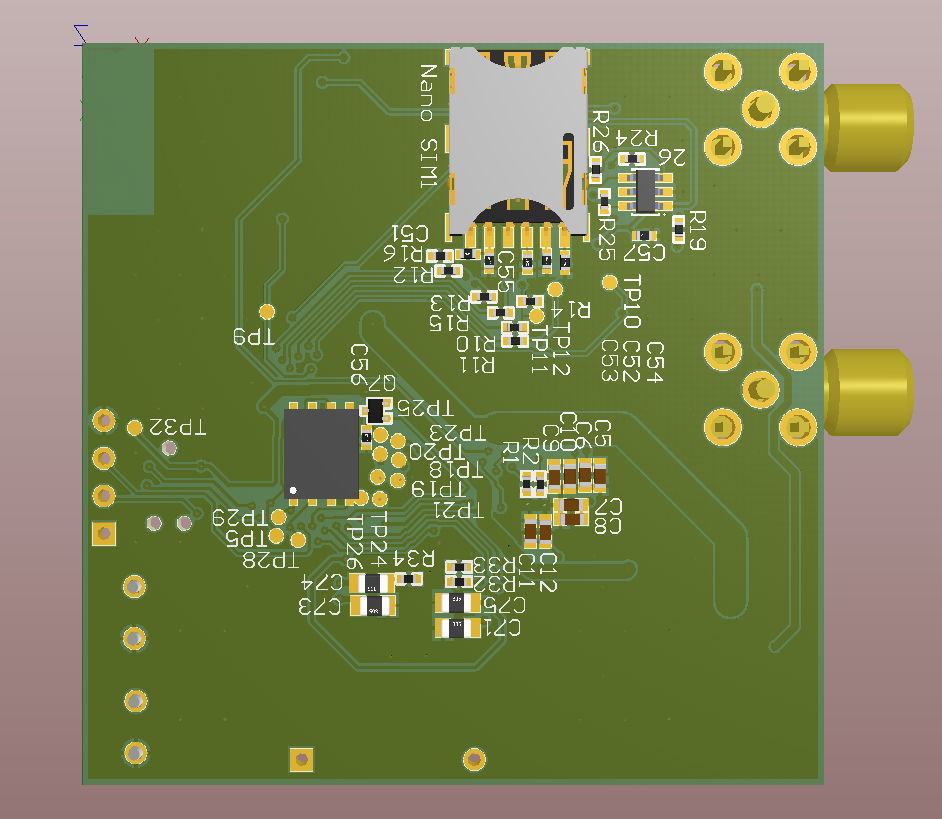
\includegraphics[width=11cm]{img/board_layouts/mainboard_visualization_bottom.png}
	}
	
	\caption{Wygląd dolnej warstwy płytki urządzenia lokalizującego oraz jej wizualizacja. \\ Źródło: Opracowanie własne.}
	\label{fig:image_mainboard_bottom_board}
\end{figure}